\documentclass[11pt]{article}
\setlength{\columnsep}{0.5cm}
\usepackage[margin=1.5cm]{geometry}
\usepackage{amsmath}
\usepackage{amsfonts}
\usepackage{stmaryrd}
\usepackage{amssymb}
\usepackage{amsthm}
\usepackage{graphicx}
\usepackage{caption}
\usepackage{subcaption}
\usepackage{algorithm}
\usepackage{algpseudocode}
\usepackage{titling}
%========================================================
\usepackage{tabularx}
\usepackage{hhline}
\usepackage{multirow}
\usepackage{diagbox}
\usepackage{slashbox}
\usepackage{array}
\usepackage{tikz,colortbl}
\usetikzlibrary{calc}
\usepackage{zref-savepos}

\newcounter{NoTableEntry}
\renewcommand*{\theNoTableEntry}{NTE-\the\value{NoTableEntry}}

\newcommand*{\notableentry}{%
  \multicolumn{1}{@{}c@{}|}{%
    \stepcounter{NoTableEntry}%
    \vadjust pre{\zsavepos{\theNoTableEntry t}}% top
    \vadjust{\zsavepos{\theNoTableEntry b}}% bottom
    \zsavepos{\theNoTableEntry l}% left
    \hspace{0pt plus 1filll}%
    \zsavepos{\theNoTableEntry r}% right
    \tikz[overlay]{%
      \draw[black]
        let
          \n{llx}={\zposx{\theNoTableEntry l}sp-\zposx{\theNoTableEntry r}sp},
          \n{urx}={0},
          \n{lly}={\zposy{\theNoTableEntry b}sp-\zposy{\theNoTableEntry r}sp},
          \n{ury}={\zposy{\theNoTableEntry t}sp-\zposy{\theNoTableEntry r}sp}
        in
        (\n{llx}, \n{lly}) -- (\n{urx}, \n{ury})
        (\n{llx}, \n{ury}) -- (\n{urx}, \n{lly})
      ;
    }% 
  }%
}

%========================================================
\usepackage{hyperref}
\hypersetup{
    colorlinks=true,    % false: boxed links; true: colored links
    linkcolor=black,     % color of internal links
    citecolor=black,     % color of links to bibliography
    filecolor=black,  % color of file links
    urlcolor=black      
     % color of external links
}
%========================================================
% Customize table reference format
\renewcommand{\tablename}{Table} % Change table name to "Table"
\renewcommand{\thetable}{\arabic{table}} % Number tables as 1, 2, 3, ...
\makeatletter
\renewcommand{\p@table}{\tablename~} % Include "Table" before the table number
\makeatother
%========================================================
\usepackage[style=numeric]{biblatex}
\addbibresource{refs.bib}
%========================================================

\newcommand{\intset}[2]{\llbracket #1, #2 \rrbracket}

\title{Critique of Unconstrained Memoryless Modular Strategies in Continual Learning}
\author{Author Name}
\date{\today}

\begin{document}





\begin{titlepage}
    \centering
    
\includegraphics[width=0.3\textwidth]{images/logo_ENS.png} \hfill % Replace 'logo1.png' with your image file
    
\includegraphics[width=0.3\textwidth]{images/logo_MVA.png} \hfill % Replace 'logo2.png' with your image file
    \vspace{1cm}
    
    
\includegraphics[width=0.3\textwidth]{images/logo_ETH.png} \hfill % Replace 'logo3.png' with your image file
    
\includegraphics[width=0.3\textwidth]{images/logo_INI.png} \hfill % Replace 'logo4.png' with your image file
    \vfill
    
    %\HRule \\[0.4cm]
    {\huge \bfseries Artificial Neurogenesis in the Context Continual Learning \\[0.4cm]} % Replace with your thesis title
    %\HRule \\[1.5cm]
    
    \textsc{\LARGE Master Masthematics, Vision et Apprentissage}\\[1.5cm] % Replace with your degree name
    
    \textsc{\Large Mathis REYMOND}\\[0.5cm] % Replace with your name
    
    \vfill
    
    \Large
    \begin{tabbing}
        \hspace{4cm} \= \textbf{Supervisor:} \hspace{1cm} \= Pr. Melika Payvand \\ % Replace with supervisor's name
        \hspace{4cm} \= \textbf{Institution:} \> University Name \\ % Replace with institution name
        \hspace{4cm} \= \textbf{Department:} \> Department Name \\ % Replace with department name
    \end{tabbing}
    
    \vfill
    
    {\large \today}\\[2cm] % Date
    
\end{titlepage}



\twocolumn[

\begin{abstract}
    %This paper is a critique of unconstrained memoryless modular strategies in continual learning. We argue that these strategies are not well-suited for the problem of continual learning, as they certainly don't solve it but at best, solve specific benchmarks. These approaches do not deal with the core challenges of distributing inputs to modules and merging outputs from modules. More fundamentally, we show that these strategies are inherently unable to tackle these challenges and that they mainly mitigate pollution between tasks. We also discuss the management of hyperparameters in continual learning, which is often unfair and can lead to overfitting on benchmarks. Finally, we propose a naive approach that reaches state-of-the-art performance on two benchmarks, highlighting the limitations of unconstrained memoryless modular strategies.
    Starting with a critical review of Elastic Weight Consolidation method (EWC), we argue that unconstrained memoryless modular strategies does not account for all dimensions of pollution which is an inherent limitation to solve continual learning. So why does the litterature seem to show positive results? The reason lies in the introduction of hyperparameters (HPs) that create trade-offs between the tasks. Therefore, we argue that EWC should not perform any better than any other approach that makes similar trade-offs. To verify this, we present naive baselines along with a more elaborated method that only make trade-offs and show that, with the same amount of hyperparameters, they achieve similar performance to EWC. Additionally, we study how performances are impacted by the amount of hyperparameters, from $O(1)$ to $O(n^2)$. However, with all these HPs, we are essentially overfitting on the benchmarks, which we demonstrate through the introduction of validation benchmarks.
\end{abstract}
\vspace{1cm}


\tableofcontents]




\section{Introduction}



\subsection{Continual learning}


We, humans are able to learn a wide variety of tasks throughout our lives. We can learn to play the piano, to speak a new language, to ride a bike, to cook a new recipe, etc. We can even learn to perform several tasks at the same time, such as playing the piano and singing at the same time. This ability to learn a sequence of tasks without forgetting the previously learned tasks is called continual learning. Continual learning is a fundamental aspect of human intelligence, and it is a key challenge in artificial intelligence. Indeed, when an artificial model using backpropagation is assigned to learn a sequence of tasks, its final state after training on a task is percieved as an initial state to train on the next task, which will be overwritten during the training procedure on the new task, leading to catastrophic forgetting of the previous task. This is a major limitation of backpropagation on neural networks, and it is a key challenge in artificial intelligence. In this paper, we will discuss the problem of continual learning and we will introduce a new approach to continual learning that is based on the idea of growing neural networks.

\vspace{2mm}
\noindent
In a very broad sense, one can define continual learning as

\begin{quote}
    \itshape
    \centering
    the problem of learning several tasks sequentially.
\end{quote}
Although this assumption is sometimes relaxed in the literature [REFLA], the fact that tasks have to be learnt \textit{sequentially} implies that once the training procedure on a task is done, its associated training data cannot be used again. 

\vspace{2mm}
\noindent
Continual learning comes in different flavors that vary depending on the working assumptions we make. Some of the most common frameworks include the following[REFLA].

\vspace{2mm}
\noindent
In \textit{Task Incremental Learning}[REFLA], the model is trained sequentially on a series of tasks, with each task involving a different set of data or objectives, such as sentiment analysis and then object classification within images. The model knows which task it is dealing with at any given time, and it often has task-specific components or outputs. This framework is very general and can be applied to a wide range of problems. Then comes \textit{Domain Incremental Learning}[REFLA] framework, within which the model faces a sequence of tasks that involve the same objective but in different domains. During inference, the model is not informed which domain it is operating in and must generalize across these domains. Finally, \textit{Class Incremental Learning}[REFLA] involves learning new classes sequentially, without task identifiers. The model is expected to classify data from any of the classes it has learned so far, even as new classes are introduced. This is often considered the most challenging form of continual learning, as the model must avoid catastrophic forgetting while continuously expanding its ability to recognize new classes.

\vspace{2mm}
\noindent
Litterature also aknwoledges other frameworks such as \textit{Lifelong Learning} [REFLA], and other classifications of these frameworks [REFLA].


\subsection{Approaches to continual learning}


The problem of continual learning has been heavily investigated in the past decade, leading to the development of various approaches to mitigate catastrophic forgetting. These approaches can be broadly categorized into regularization-based, replay-based and architectural.

\vspace{2mm}
\noindent
\textit{Regularization-based} approaches, which constrain the learning process through a regularization term embedded in the loss function, aim at preventing drastic changes to model parameters that are critical for previous tasks. Fundational methods to this category of approaches include Elastic Weight Consolidation (EWC) [REFLA], which estimates the importance of each parameter and penalizes changes accordingly, and Synaptic Intelligence (SI) [REFLA], which dynamically accumulates information about parameters importance throughout training of all the tasks.

\vspace{2mm}
\noindent
Another important approach is \textit{replay-based learning}, which involves storing or generating data from previous tasks to revisit during the training of new tasks. This helps maintain performance on older tasks by refreshing the model's memory of past data. Methods like Experience Replay [REFLA] store a small buffer of past samples which are forwarded to the model when training on new tasks, while Generative Replay [REFLA] uses a external generative model to recreate as many data from previous tasks as needed. 

\vspace{2mm}
\noindent
Finaly, \textit{architectural approaches} modify the model's structure to accommodate new tasks while preserving knowledge from previous ones. Methods like Progressive Neural Networks (PNN) [REFLA] add new subnetworks for each task, allowing forward knowledge transfer from old tasks dedicated subnetworks, while keeping the new ones isolated. Conversely, Mixture of Expert Models [REFLA] leverage a gating system which is designed to identify and distribute tasks to expert subnetworks.

\vspace{2mm}
\noindent
However, these categories do not constitute a proper partition of the litterature as they are not mutually exclusive. Approaches such as Architectural and Regularization 1 (AR1) [REFLA] fall both in regularization-based and architectural categories. Additionally, these categories do not encompass certain methods such as adversarial approaches [REFLA].


\subsection{Our specific framework}


Given the variety of frameworks and approaches, we need to narrow down and specify ours. In previous subsections, we introduced frameworks and approaches to continual learning through categories. But beyond these categories, which provide a useful overview of the literature, what truly matters are the specific assumptions under which we operate.

\vspace{2mm}
\noindent
First, we will focus on classification tasks involving the same set of classes. We assume that the model is notified when transitioning to the training of a new task. Each task must be handled strictly sequentially, meaning we do not permit any use of data from previous tasks. Additionally, we assume the total number of tasks is unknown and cannot be leveraged during the learning process.

\vspace{2mm}
\noindent
As for the methods, our approach will be \textit{modular}, meaning it will break down the learning process into subproblems and explicitly leverage dedicated modules to address these subproblems. These modules may consist of independent subnetworks, subnetworks that share some parameters, or groups of neurons distributed within the entirer network.

\vspace{2mm}
\noindent
On the top of the modularity of our approach, we make to additional assumptions regarding the way we will process information. First, we will work with \textit{unconstrained} architectures, meaning that we will not impose any architectural constraint on the model that could allow the processing or implicit remembering of the specificities of the past task. To this regard, convolutional or graph neural networks are out of our scope. We will also work with \textit{memoryless} strategies, meaning that in addition to banning the use of data from previous tasks, we will not allow to leverage a replay buffer or generative rehearsal module.

%focus on unconstrained and memoryless strategies. This means that we will not impose any constraint on the learning process that could allow the processing or implicit remembering of the specificities of the past task, and that we will not use any memory of the past tasks. Finally, we will decompose the learning process into subproblems, which will be solved independently. This will allow us to focus on the processing of the subproblems and the merging of the solutions of the subproblems to form the solution of the original problem.



\section{Our approach : GroHess}



\subsection{Motivation}


\begin{figure}
    \centering
    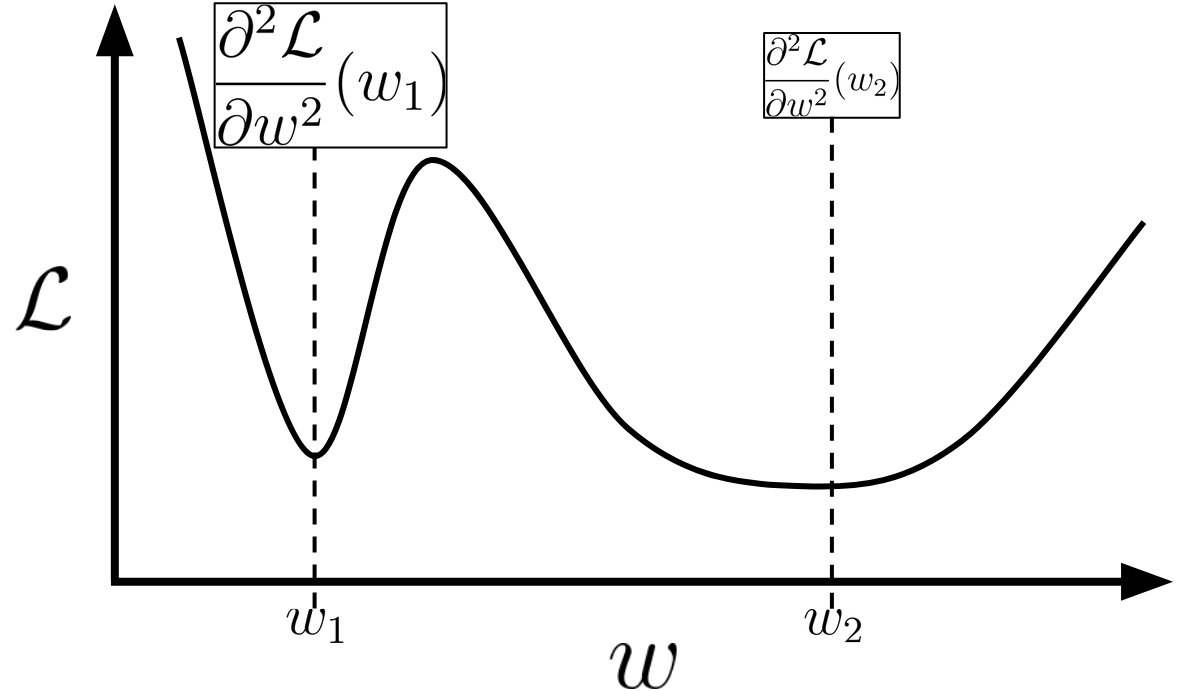
\includegraphics[width=0.40\textwidth]{images/motivation_GroHess.png}
    \caption{Illustration of our sense of importance of weights. When the second derivative of the loss with respect to a weight is high, the weight is considered important as modifying even a little bit would lead to a significant change in the loss. However, when the second derivative is low, modify the weight has little impact on the loss.}
    \label{fig:motivation_GroHess}
\end{figure}

To address the problem of Continual Learning, one approach is to train independent specialized modules and a gating system that learns to recognize tasks, similar to Mixture of Experts Models [REFLA]. However, the tasks to be learned often have redundant features that we would like to leverage, so that only the new features of a task are learned without forgetting the old ones. The emergence of such features relies on constraints, starting with imposing small size of the model. Therefore, we would prefer to start training with a model of moderate size and expand it as more tasks are introduced.


\vspace{2mm}
\noindent
Such an approach presents several challenges. First, it requires to determine which important features to retain. Then, we must figure out how to retain them. Finally, we need to determine how to use them to handle new tasks. To achieve this, we introduce GroHess, a new approach to architecture growth in the context of continual learning. GroHess is based on the idea of growing the model by adding new neurons to the model when the importance of a weight is high, as determined by the second derivative of the loss with respect to the weight. This is illustrated in \ref{fig:motivation_GroHess}. When the second derivative of the loss with respect to a weight is high - such as in $w_1$ - the weight is considered important as modifying it even a little bit would lead to a significant change in the loss. Conversely, when the second derivative is low - such as in $w_2$ - modifying the weight has little impact on the loss. This allows us to determine which weights are important and which are not, and to grow the model accordingly.



\subsection{Description}


More specifically, We control the growth of the model through two percentiles : the gradient percentile and the Hessian percentile. These percentiles allow us to define what is considered to be "high", relatively to the other weights first and second derivatives.

\vspace{2mm}
\noindent
Once the training procedure on a task is done, we compute the second derivative of the loss with respect to each weight through all the data batches of the task. When the second derivative of a given weight with respect to the loss falls above the hessian percentile, comparatively to the second derivate of the other weights, it means that modifying this weight will strongly disturb what has been learnt on the task. Thus, we compute a bianry mask recording which weights are important for the task according to the second derivative. Conversely, when training on a task, if the loss start to stagnate, we take a look at the last computed gradient with backpropagation. If the gradient of a given weight falls above the gradient percentile, comparatively to the other gradients, it means that according to backpropagation, this weight has to be strongly updated. As a consequence, when both the first and the second derivatives of a given weight are high, we have a tension that leads us into growing a new neuron, to accodmodate both backpropagation and the preservation of the knowledge of the task. The weight we grow from is then frozen, it wont be updated ever again, but we will keep backpropagating gradients through it. 

\vspace{2mm}
\noindent
Everytime one grows a neuron, this neuron has to be initialized, which means that 6 choices have to be made : the value of its bias, the value of the incoming weights, and the value of the outgoing weights and their respective gradients. The meaning of a growth is allow both the preservation of the knowledge of the task and the learning of the new task. As a consequence, we mostly copy the neuron we are growing from, and we only set the outgoing weights whose first and second derivatives were not both high to zero. This choice is motivated by the fact that we don't want the new neuron to disrupt the learning process.


\begin{algorithm*}
    \caption{Training GroHess on $n$ tasks}
    \begin{algorithmic}[1]
    \State \textbf{Input:} \\
    - Model $\Sigma_{ini}$ \\ 
    - List of $n$ tasks $L = [(X_1,Y_1), \ldots, (X_n,Y_n)]$\\
    - Hessian percentile $\tau_{hessian}$ \\
    - Gradient percentile $\tau_{gradient}$
    \State \textbf{Output:} Trained model $\Sigma_{fin}$ solving each task
    \State
    
    \State \textbf{Step 1:} Train $\Sigma_{ini}$ on $(X_1,Y_1)$
    \State \textbf{Step 2:} Compute $\nabla^2_{\Sigma_{ini}} \mathcal{L}_{(X_1,Y_1)}$ for each weight and define the binary mask $\mathcal{M}_{hessian}$ using $\tau_{hessian}$  
    \For{each reamining task $(X_i,Y_i)$}
        \For{each batch $(x_i,y_i)$ in $(X_i,Y_i)$}
            \State \textbf{Step 3:} Perform training step on $(x_i,y_i)$
            \If{loss stagnates}
                \State \textbf{Step 4:} Compute $\nabla_{\Sigma_{ini}} \mathcal{L}_{(x_i,y_i)}$ and define the binary mask $\mathcal{M}_{gradient}$ using $\tau_{gradient}$
                \State \textbf{Step 5:} Compute the binary mask $\mathcal{M}_{overlap}$ as the element-wise product of $\mathcal{M}_{hessian}$ and $\mathcal{M}_{gradient}$
                \State \textbf{Step 6:} Grow as many neurons on $\Sigma_{ini}$ as $\mathcal{M}_{grow}$ has column with at least a $1$
                \State \textbf{Step 7:} Freeze the weights we just grew from
            \EndIf
        \EndFor
        \State \textbf{Step 8:} Compute $\nabla^2_{\Sigma_{ini}} \mathcal{L}_{(x_i,y_i)}$ and update $\mathcal{M}_{hessian}$ using $\tau_{hessian}$
    \EndFor
    \end{algorithmic}
\end{algorithm*}


\begin{figure*}
    \centering
    \begin{subfigure}[b]{0.4\textwidth}
        \centering
        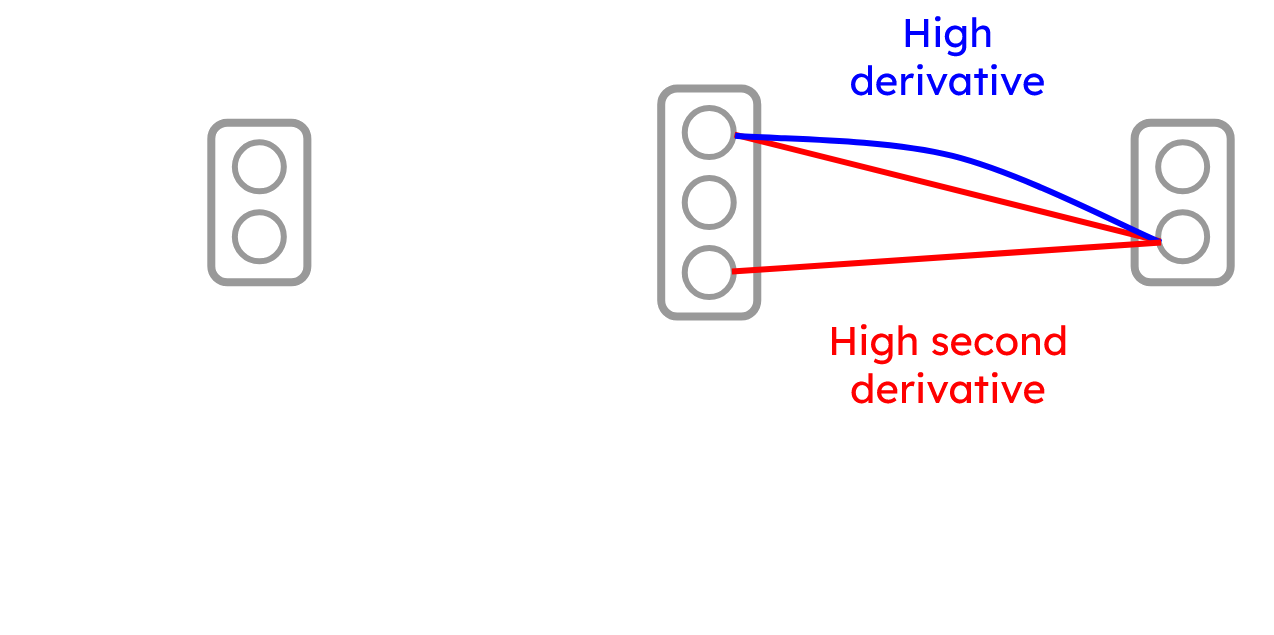
\includegraphics[width=0.95\textwidth]{images/GroHess_explication_1.png}
        \caption{Hessian mask is computed at the end of training on task $n-1$ and Gradient mask is computed during training on task $n$.}
        \label{fig:GroHess_explication_1}
    \end{subfigure}
    \hspace{-0mm}
    \begin{subfigure}[b]{0.4\textwidth}
        \centering
        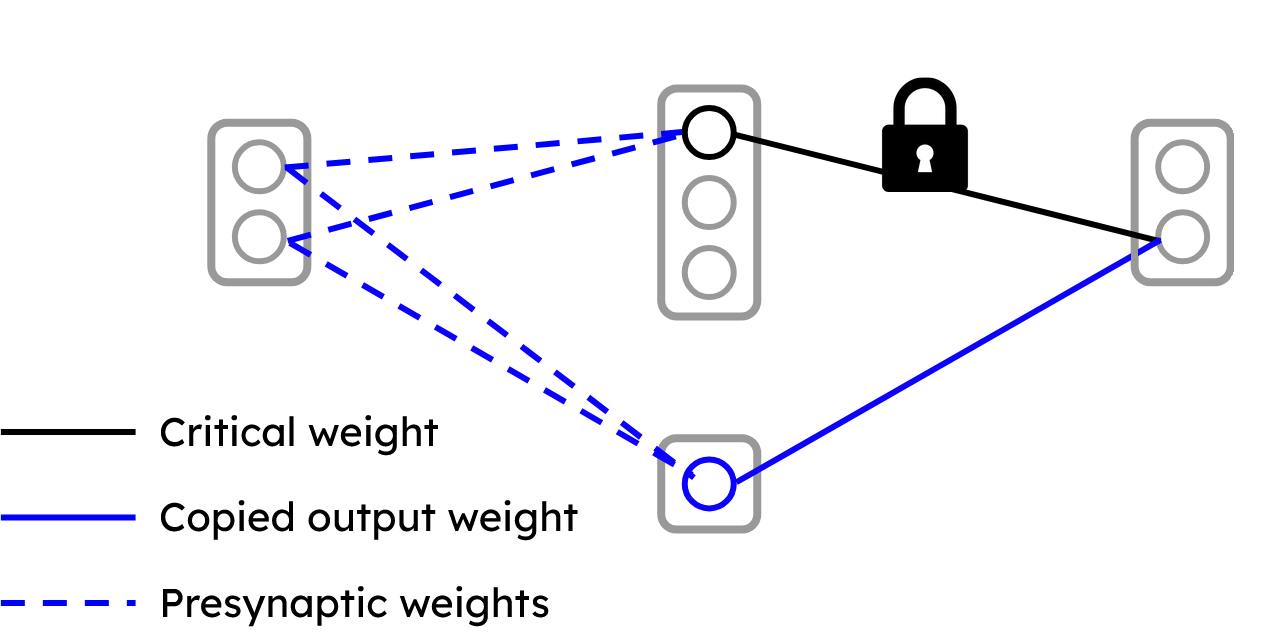
\includegraphics[width=0.95\textwidth]{images/GroHess_explication_2.png}
        \caption{The important weight is frozen and a new neuron is grown from it.}
        \label{fig:GroHess_explication_2}
    \end{subfigure}
    \caption{Illustration of the GroHess procedure.}
\end{figure*}



\subsection{Baselines}


Our method is based on two ideas : a hessian-inspired mechanism to define weights importance and a growth mechanism to add new neurons to the model. To evaluate the relevance of these ideas, we introduce several baselines.

% Doing nothing initial size
% Doing nothing mean final size
% Growing without GroHess
% Using GroHess to freeze important weights without growing

To evaluate the effectiveness of our method, which incorporates a Hessian-inspired mechanism for determining weight importance and a growth mechanism for adding new neurons to the model, we introduce four baselines.

\vspace{2mm}
\noindent
In a first "vanilla" baseline, we define a model in the same initial configuration as the one used optimized with GroHess. During the training procedure through the tasks, no additional neurons are added, and no special mechanism is used to adjust or freeze weights according to their importance for the tasks. The model remains at its original size throughout the training process.

\vspace{2mm}
\noindent
We also train a second "vanilla" baseline, but the initial size of its hidden layers is that of the average final hidden layer sizes when training with GroHess. So, from the beginning, this baseline is in the average configuration of a model trained with GroHess. 

\vspace{2mm}
\noindent
We also design a third baseline, where perform growth without GroHess, during the training procedure. This baseline involves starting the training process on the first task with a model of the same size as the one used with GroHess. However, everytime the model moves to training on a new task, it blindly adds new neurons to each layer, randomly initialezed, and without freezing any weight. This baseline helps evaluate the benefits of our approach of defining weights importance through Hessian coefficients. 

\vspace{2mm}
\noindent
Finally, our fourth and last baseline uses GroHess to freeze important weights without triggering the growing mechanism.This baseline is initialized in the same way as the second one, however, we leverage GroHess to freeze important weights during the training process, but without growing new neurons as GroHess would normaly do. This baseline is supposed to isolate the effectiveness of the growing mechanism to improve perfomances.

\vspace{2mm}
\noindent
These baselines allow us to thoroughly analyze the contribution of the two main mechanisms of our approach, namely the Hessian-inspired weight importance mechanism and the growth mechanism, independently and in combination.



\section{Main experiment}



\subsection{Permuted MNIST}


\begin{figure*}
    \centering
    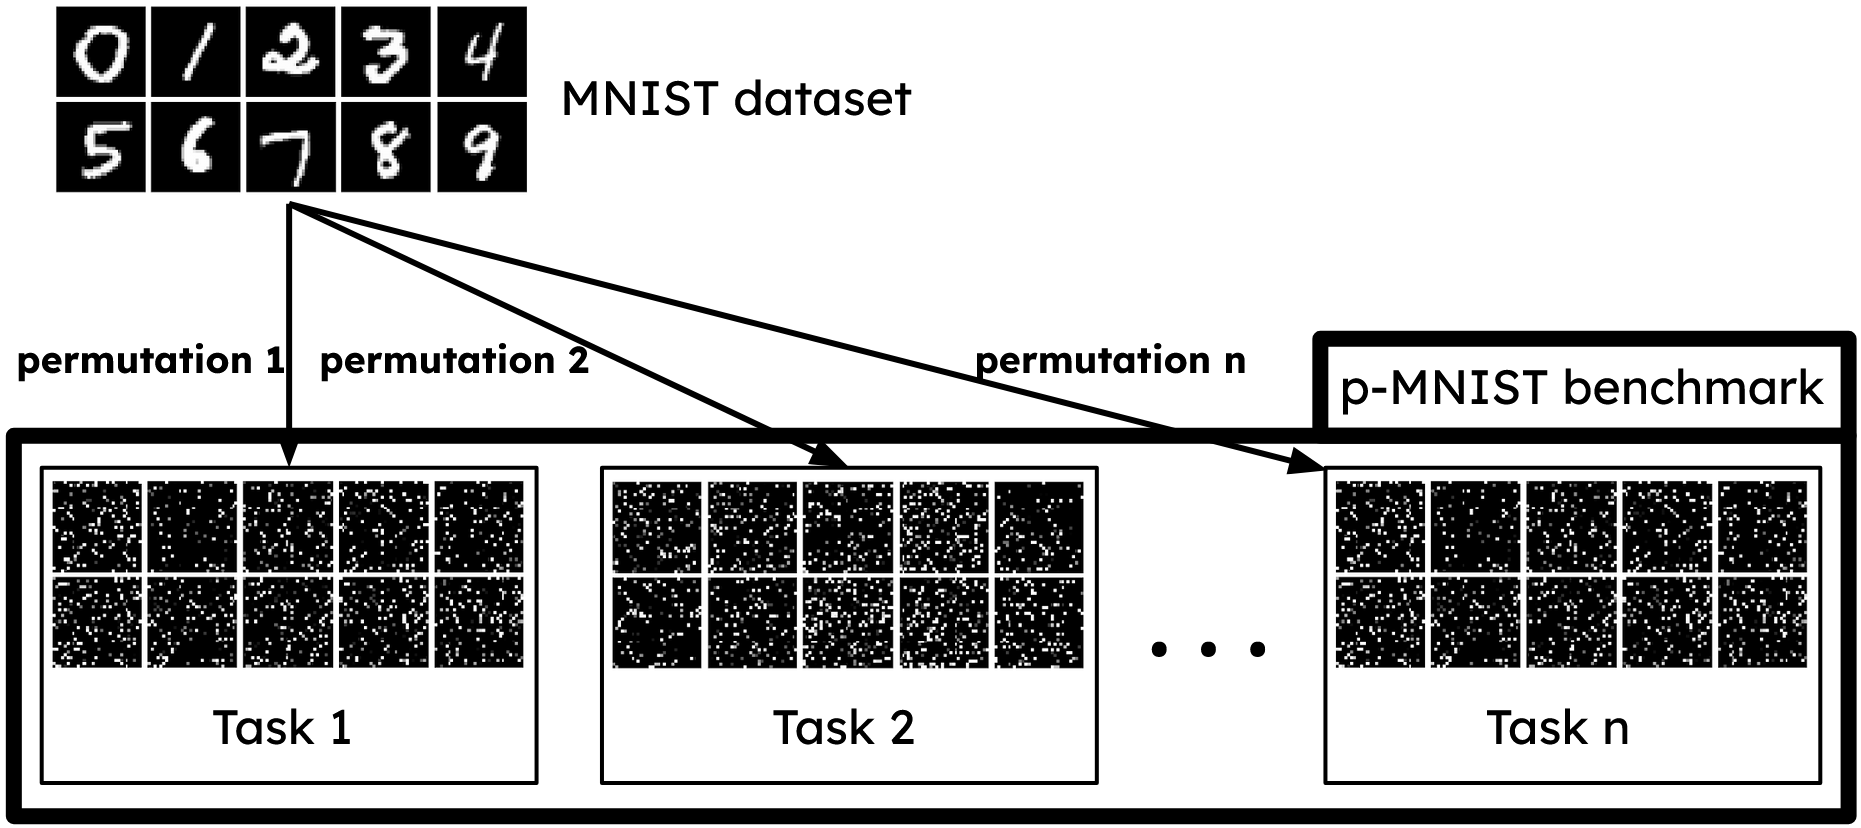
\includegraphics[width=0.65\textwidth]{images/p-MNIST.png}
    \caption{Illustration of the process of creating a p-MNIST benchmark.}
    \label{fig:p-MNIST}
\end{figure*}

A permuted MNIST (p-MNIST) dataset [REFLA] is a variant of the classic MNIST dataset where images are transformed through a fixed random permutation of pixel positions, creating a shuffled version of each original image. The label associated with each image remains the same, meaning the digits themselves are unchanged, but their visual structure is modified. Then, a p-MNIST task is define as solving the classification problem associated to a p-MNIST dataset. As each p-MNIST dataset is generated by a different permutation of MNIST dataset, there are $784!$ possible p-MNIST datasets and as many p-MNIST tasks. Finally, a p-MNIST benchmark is created by selecting a subset of these tasks. See \ref{fig:p-MNIST} for illustration.

\vspace{2mm}
\noindent
Permuted MNIST is particularly significant in the context of continual learning as it offers the opportunity to generate arbitrary long sequences of tasks with a fixed number of classes and a fixed number of samples per class. Additionally, users have a great control over the difficulty of a benchmark, which is directly associated with the similarity of the permutations used to generate the tasks of the benchmark. Finally, the p-MNIST benchmark is a well-established benchmark in the continual learning literature, which allows for comparison of different approaches.

\vspace{2mm}
\noindent
On the other hand, litterature has come with a lot of criticism about the p-MNIST benchmarks. First, they are rather simple benchmarks, which do not reflect the complexity of real-world tasks. Second, the random permutations break the spatial structure of images we can find in the real world, which means that the p-MNIST benchmarks are not well-suited to evaluate method that require spatial reasoning on tasks such as object detection or segmentation. In particular, the permutations of pixels disrupt with the assumption of locality and translation invariance which are at the basis of convolutional neural networks. As a consequence, approaches leveraging convolutional neural networks are disadvantaged on p-MNIST benchmarks.

\vspace{2mm}
\noindent
Despite this criticism, we have chosen to use p-MNIST benchmarks. They are relevant for our study of GroHess as their very simplicity allows to understand the fundamental principles of our exploratory method. Additionally, the ability to generate not only several tasks, but also several comparable benchmarks will allow us to motivate and introduce a validation paradigm in continual learning.


\subsection{Training protocol}


Our model consist in a multi layer perceptron with 2 hidden layers (or 3 layers in total). Input and output sizes are 784 and 10 respectively. Each hidden layer contains initialy contains 300 neurons. The growth of the model happens from the output layer, which means that when a weight has both a high first and second derivatives, we grow a neuron on the layer preceeding it (in the forward sense). We control the growth of the model through two percentiles : the gradient percentile and the Hessian percentile. When both first and second derivative of the loss with respect to a weight are above the gradient and Hessian percentiles, respectively, we grow a new neuron. 

\vspace{2mm}
\noindent
We train our models following GroHess algorithm on a sequence of $10$ p-MNIST tasks, each with the usual $10$ MNISTS classes. For each task $80\%$ of the train set is used for training, $20\%$ is used for validation and $100\%$ of the test set is used to test the model. We train GroHess with the Adam optimizer and the cross-entropy loss. For each task, the number of epochs and the learning rate are left as optimizable hyperparameters. We use a batch size of $128$. See \ref{table:HPs} for the complete list of hyperparameters.


\begin{table}[h!]
    \centering
    \begin{tabular}{|l|c|}
    \hline
    \multicolumn{2}{|c|}{\textbf{Hyperparameters (HPs)}} \\
    \hline
    \textbf{Fixed HPs} & \textbf{Value}\\
    \hline
    Number of Layers & 3 \\
    Initial hidden layers size & 300 \\
    Batch Size & 128 \\
    Optimizer & Adam \\
    Loss & Cross-entropy \\
    Growth happens from & Output \\
    Gradient percentile & 0.98 \\
    Hessian percentile & 0.98 \\
    \hline
    \hline
    \textbf{Optimized HPs} & \textbf{Range}\\
    \hline
    Learning Rate & 1e-5 - 2e-3 \\
    Number of epochs & 2 - 10 \\
    \hline
    \end{tabular}
    \caption{Hyperparameters value or range}
    \label{table:HPs}
\end{table}


As the training loop is called once for each task, it means that a learning rate and number of epoch have to be found through hyperparameter optimization (HPO) for each task. HPO is performed using the Optuna library [REFLA] with the Tree Parzen Estimator (TPE) algorithm. We use the validation set to evaluate the performance of the model and to optimize the hyperparameters. We use the average accuracy over all tasks as the metric to optimize. We perform HPO for each task sequentially, meaning that once the best hyperparameter values for a task are found, we retrain the model with them before moving to the next task. We repeat this process $10$ times with random seeds 88 to 92 and we report the average test accuracy over all runs.



\section{Results}



\begin{figure*}
    \centering
    \begin{subfigure}[b]{0.35\textwidth}
        \centering
        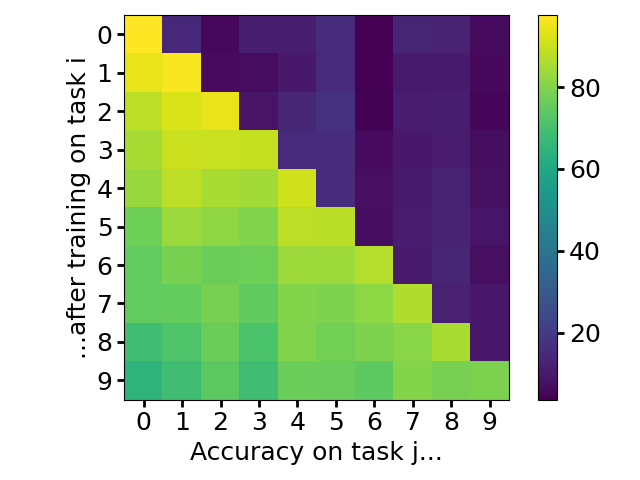
\includegraphics[width=0.95\textwidth]{images/accs_matrix.png}
        \caption{Test accuracy on each task as GroHess move forward through the tasks}
        \label{fig:test_accs_matrix}
    \end{subfigure}
    \hspace{-0mm}
    \begin{subfigure}[b]{0.35\textwidth}
        \centering
        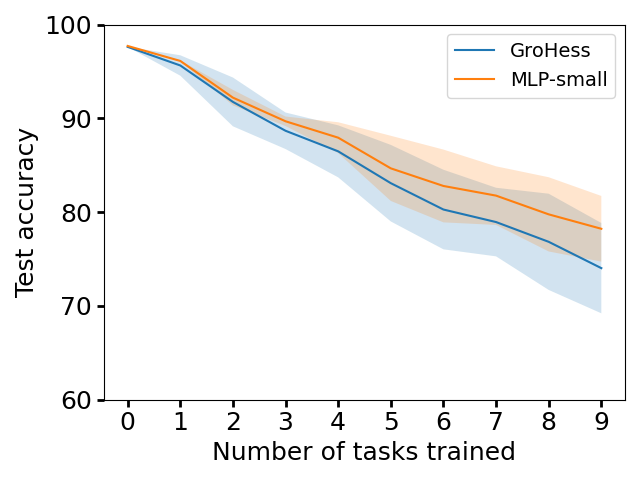
\includegraphics[width=0.95\textwidth]{images/agg_avg_acc_curve.png}
        \caption{Average test accuracy on tasks trained so far}
        \label{fig:classic_plot}
    \end{subfigure}
    \caption{Evolution of the average test accuracy during training. The plots show the average test accuracy over all runs on seed 88 to 92. \ref{fig:classic_plot} also represents the standard deviation over runs.}
\end{figure*}

In \ref{fig:test_accs_matrix}, we show the test accuracy on each task as GroHess move forward through the tasks. This visualization provides a better insight than aggregated metrics as it allows us to inspect directly the performance of the model on each task during training. An interested feature of our method is that the coefficients below the diagonal of the matrix, on the same line are relatively equal, which means that our GroHess is able to retain knowledge of the previous tasks without completely overwritting them. Additionally, we observe that column-wise, the accuracy is decreasing, which is reasonnable : as the model learns tasks, it has to remember more past tasks, which makes the learning process harder.

\vspace{2mm}
\noindent
Additionnaly, \ref{fig:classic_plot} shows the average test accuracy on tasks trained so far. In other words, the value associated to abscisse $i$ is the average of the coefficients below the diagonal of the $i^{th}$ line of the matrix in \ref{fig:test_accs_matrix}. This plot is a more classical way to represent the performance of the model as it moves forward through the tasks, as it shows the ability of the approach to learn the first tasks of the benchmark. The last point of this plot represent the average test accuracy over all tasks, once the model has been trained on all of them.


\begin{figure*}
    \centering
    \begin{subfigure}[b]{0.4\textwidth}
        \centering
        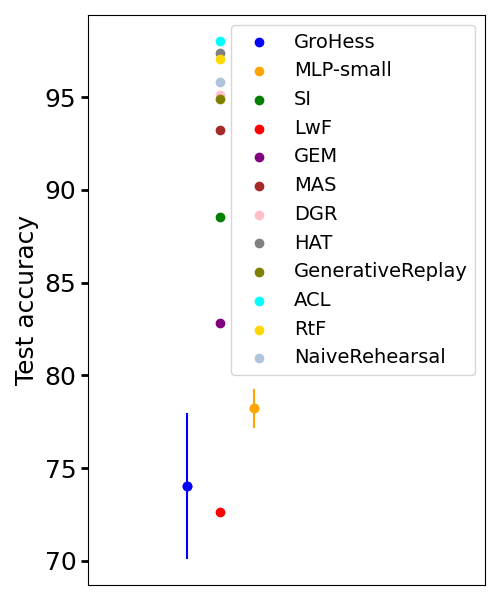
\includegraphics[width=0.75\textwidth]{images/lit.png}
        \caption{Our results, along with results collected in the litterature on the 10 tasks p-MNIST benchmark [REFLA].}
        \label{fig:results}
    \end{subfigure}
    \hspace{-0mm}
    \begin{subfigure}[b]{0.4\textwidth}
        \centering
        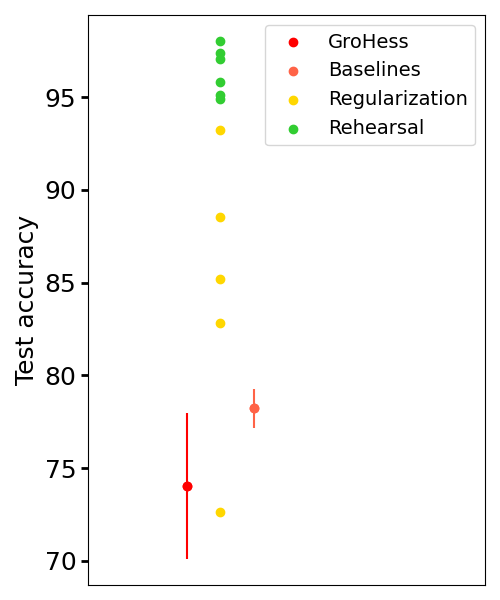
\includegraphics[width=0.75\textwidth]{images/lit_grouped.png}
        \caption{Same results as in \ref{fig:results}, but grouped by type of approach.}
        \label{fig:results_grouped}
    \end{subfigure}
    \caption{Results}
\end{figure*}

Additionally, we present the results obtained with GroHess along with a comparison to litterature in \ref{fig:results}. We also compare our approach to the baselines we introduced in the previous section. Each dot in this plot represent the average accuracy over all tasks of a p-MNIST benchmark after training on all of them sequentially. For both our methods and the methods reproduced, the error bars represent the standard deviation over runs on seed 88 to 92. The permutations used to generate the p-MNIST tasks are the same for all the methods we ran, namely the first permutation as suggested by the random module of numpy when provide seeds 1 to 10.

\vspace{2mm}
\noindent
Then, we group the results by type of approach in \ref{fig:results_grouped}. We identify detached groups. The methods relying on replay-based learning or rehearsal are performing much better than the other methods. The performances of the regularization methods are more spread, but they are generally better than our baselines and GroHess.



\section{Paradigmatic discussion}



\subsection{Hyperparameters optimizations}


In the section in which the training protocol is introduced, we suggested to have only two hyperparameters, the number of epochs and the learning rate. However, as we mentionned, we performed one HPO for each task we train our model on. As consequence, despite having two hyperparameters, we end up with $10$ values for each of them, which means that the whole training procedure on the benchmark carries $20$ hyperparameters. 

\vspace{2mm}
\noindent
Continual learning enables several ways to manipulate hyperparameters. In this subsection, we will discuss various approaches to manipulate them. 

\vspace{2mm}
\noindent
Let's introduce a hyperparameter $\lambda$. One could set this hyperparameter to be the same for all the tasks, which would result in a total of $1$ hyperparameter. To set the value of this hyperparameter, one could perform a single HPO on the first task, and keep using the same value for the forecoming task. However, when proceeding that way, the hyperparameter is not optimized for each task, only for the first one. Therefor, this way of performing HPO is not suited for our continual learning framework. In order to keep $\lambda$ to only one value while optimizing it on all the tasks, one could perform a single HPO on the whole benchmark. That means that once a value for $\lambda$ is suggested by the HPO algorithm, we would train through all the tasks using this value. At the end of the HPO, we would end up with a single value of $\lambda$ that would be tuned for all the tasks. However, optimizing in such a way require to have access to all the tasks at the same time, which breaks the continual learning framework. Indeed the value of $\lambda$ used when training on the first task as to be decided before accessing data from the latter tasks. This way of performing HPO is highly problematic as it causes data leakage. That is why we refere to it as a cheated HPO with respect to continual learning framework. See [\ref{tab:HPOs}] top-left.

\vspace{2mm}
\noindent
Alternatively, one could set this hyperparameter to a specific value $\lambda_i$ for each task $i$, this would require to perform an HPO on each task and would result in a total of $n$ hyperparameters. This way of performing HPO is suited for continual learning framework, as tasks are treated strictly sequentially. This is how we proceeding when training with GroHess and it is also the most common approach to HPO in the litterature. See [\ref{tab:HPOs}] bottom-center. As optimizing for the value of $\lambda_{i+1}$ requires to have the value of $\lambda_i$, we refere to this approach as greedy HPO.

\vspace{2mm}
\noindent
Remarkably, one could merge both of the previous approaches is a cheated HPO with $n$ parameters. This would require to perform a single HPO on the whole benchmark, but instead of suggesting a single value of $\lambda$ at each trial, the HPO algorithm would suggest values $\lambda_1,...,\lambda_n$, one for each task $i$. This way of performing HPO is even more problematic than the first way as it combines data leakage and a rather high number of hyperparameters. See [\ref{tab:HPOs}] top-center.

\vspace{2mm}
\noindent
Finally, some methods in the literature introduce a hyperparameter $\lambda$ that is explicitly used to make tradeoffs between how much the model should learn from the new task versus how much it shoud retain from the previous tasks [REFLA]. Such a hyperparameter can be optimized as describded above, but it may also be used to perform tradeoffs directly between tasks. For instance, when training on task 2, one could have a $\lambda_{2,1}$ that would be used to make tradeoffs between how much the model should learn from task 2 and how much it should remember from task 1. When moving to task 3, one could have a $\lambda_{3,1}$, to tune how much the model should learn from task 3 and how much it should remember from task 1 along with a $\lambda_{3,2}$ for how much the model should learn from task 3 versus how much it should remember from task 2. More generally, one could even set a different value for this hyperparameter for each pair of tasks, meaning that one could introduce $\lambda_{i,j}$ for mitigating catastrophic forgetting of task $j<i$ when learning task $i>1$. Ultimately, this would result in a total of $\frac{(n-1)n}{2}$ hyperparameters. Similarly to the HPO with $n$ hyperparameters, this way of performing HPO could fit the continual learning framework, see [\ref{tab:HPOs}] bottom-right, but it could also be done is a cheated way, see [\ref{tab:HPOs}] top-right.

%The perspective of most papers is to introduce a hyperparameter at the task-level, generaly in the loss used to train on a task. That is, they write the loss used while training on task 1 and the loss used for training on task 2, where they introduce the hyperparameter. This hyperparameter appears as an attempt to control the trade-off between the importance of the new task and the importance of the old tasks. However, they remain fuzzy about what happen to this hyperparameter on the latter tasks and the way to choose the value for the hyperparameter. 

%hyperparameters $\it{i.e.}$ $O(n^2)$ hyperparameters. Thus, it appears that the fuzziness of authors about the precise number of hyperparameters is not a minor issue as it can lead to very different hyperparameters manipulation. 

%Not only is the number of hyperparameters introduced by the authors not clear, but also the way they are chosen. If they introduce only $1$ hyperparameter, that is the same for all tasks, then in the best case, it is chosen by hand, which is a very bad practice. In this case, the authors should at least explain why they chose this value or provide a heuristic, which is often not the case. In the worst case, they choose this hyperparameter through a hyperparameter optimization over all the tasks $-$ see [\ref{tab:HPOs}] top-left $-$ which is highly problematic due to data leakage. This breaks the continual learning framework as, after deployement, one has to decide the value of the hyperparameter when training on task $2$ without accessing data from the latter tasks to help deciding. This is considered cheating in the context of continual learning. However, it seems that several papers are doing so. The same could be performed with in the $O(n)$ and $O(n^2)$ hyperparameters scenarios $-$ see [\ref{tab:HPOs}] top-middle and top-right $-$ which would be even more problematic, but as it looks even more obviously problematic, it seems that no one had the idea to do so.

%In the three cases discussed above, we considered a single HPO performed on the training through all tasks simultaneously, which we regard as unfair. An alternative approach is to perform an HPO for each task individually, in a greedy fashion. This approach assumes at least one hyperparameter by task, so $O(1)$ hyperparameters is not suited $-$ see [\ref{tab:HPOs}] bottom-left. This approach enables defining $O(n^2)$ hyperparameters $\lambda_{i,j}$ for mitigating catastrophic forgetting of task $j<i$ when learning task $i>1$, where one performs an HPO on task $i$ once the model is already trained on tasks $j<i$, before moving to task $i+1$ $-$ see [\ref{tab:HPOs}] bottom-right. However, we argue that it represents to many parameters, and makes questionnable the sacalability of this approach. Additionnaly, it is likely to lead to an overfitting on benchmark through over-specificity of tradeoffs. Finally the most reasonable approach seems to perform an HPO on each task individually, in a greedy fashion, but with only $O(n)$ hyperparameters, one for each task $-$ see [\ref{tab:HPOs}] bottom-middle. This approach is compatible with the continual learning framework, as setting the hyperparameter for training on task $i$ can be done without accessing data from the latter tasks.

\begin{table*}[h!]
    \centering
    \resizebox{\textwidth}{!}{
    \begin{tabular}{|c|c|c|c|}
        \hline
        \diagbox{Number of HPOs}{Number of HPs} & $O(1)$ & $O(n)$ & $O(n^2)$ \\ \hline
        $1$ cheated HPO
        & 
        \centering
        \begin{tabular}{cc}
            \begin{tabular}{|ccc|}
                \hline
                $T_1$ & $\cdots$ & $T_m$ \\ \hline
                \multicolumn{3}{|c|}{$\{\lambda\}$} \\ \hline
            \end{tabular}
            &
            \hspace{-5mm}
            \begin{tabular}{c}
                                                        \\
                                                        \\
                                                        \\
                \hspace{-1.5mm}\footnotesize{$HPO$}\\
            \end{tabular}
        \end{tabular}
        & 
        \centering
        \begin{tabular}{cc}
            \begin{tabular}{|ccc|}
                \hline
                $T_1$ & $\cdots$ & $T_m$ \\ \hline
                \multicolumn{3}{|c|}{$\{\lambda_1,...,\lambda_n\}$} \\\hline
            \end{tabular}
            &
            \hspace{-5mm}
            \begin{tabular}{c}
                                                        \\
                                                        \\
                                                        \\
                \hspace{-1.5mm}\footnotesize{$HPO$}\\
            \end{tabular}
        \end{tabular}
        &
        \begin{tabular}{cc}
            \begin{tabular}{|ccc|}
                \hline
                $T_1$ & $\cdots$ & $T_m$ \\ \hline
                \multicolumn{3}{|c|}{$\left\{\lambda_{i,j}|\forall 2\leq j<i\leq n\right\}$} \\\hline
            \end{tabular}
            &
            \hspace{-5mm}
            \begin{tabular}{c}
                                                        \\
                                                        \\
                                                        \\
                \hspace{-1.5mm}\footnotesize{$HPO$}\\
            \end{tabular}
        \end{tabular}
        \\ \hline
        $n$ greedy HPOs
        & 
        \notableentry 
        &
        \centering
        \begin{tabular}{cccccc}
        %    \begin{tabular}{|c|}
        %        \hline
        %        $T_1$    \\\hline
        %        $\emptyset$  \\\hline
        %    \end{tabular}
        %    &
        %    \hspace{-6mm}
        %    \begin{tabular}{c}
        %                                            \\
        %        \hspace{2mm} $\longrightarrow$      \\
        %                                            \\
        %                                            \\
        %    \end{tabular}
        %    &
        %    \hspace{-4mm}
            \begin{tabular}{|c|}
                \hline
                $T_1$    \\\hline
                $\{\lambda_1\}$  \\\hline
            \end{tabular}
            &
            \hspace{-6mm}
            \begin{tabular}{c}
                                                                            \\
                \hspace{2mm} $\longrightarrow$ \ldots $\longrightarrow$       \\
                                                                            \\
                \hspace{-14mm}\footnotesize{$HPO_1$}                          \\
            \end{tabular}
            &
            \hspace{-4mm}
            \begin{tabular}{|c|}
                \hline
                $T_n$    \\\hline
                $\{\lambda_n\}$  \\\hline
            \end{tabular}
            &
            \hspace{-6mm}
            \begin{tabular}{c}
                                                    \\
                                                    \\
                                                    \\
                \hspace{-1.5mm}\footnotesize{$HPO_n$}\\
            \end{tabular}
        \end{tabular}
        & 
        \begin{tabular}{cccccc}
        %    \begin{tabular}{|c|}
        %        \hline
        %        $T_1$    \\\hline
        %        $\emptyset$  \\\hline
        %    \end{tabular}
        %    &
        %    \hspace{-6mm}
        %    \begin{tabular}{c}
        %                                            \\
        %        \hspace{2mm} $\longrightarrow$      \\
        %                                            \\
        %                                            \\
        %    \end{tabular}
        %    &
        %    \hspace{-4mm}
            \begin{tabular}{|c|}
                \hline
                $T_2$    \\ \hline
                $\{\lambda_{2,1}\}$ \\ \hline
            \end{tabular}
            &
            \hspace{-6mm}
            \begin{tabular}{c}
                                                    \\
                \hspace{2mm} $\longrightarrow$      \\
                                                    \\
                \hspace{-3mm}\footnotesize{$HPO_2$} \\
            \end{tabular}
            &
            \hspace{-4mm}
            \begin{tabular}{|c|}
                \hline
                $T_3$    \\ \hline
                $\{\lambda_{3,1},\lambda_{3,2}\}$ \\ \hline
            \end{tabular}
            &
            \hspace{-6mm}
            \begin{tabular}{c}
                                                                              \\
                \hspace{2mm} $\longrightarrow$ \ldots $\longrightarrow$       \\
                                                                              \\
                \hspace{-14mm}\footnotesize{$HPO_3$}                          \\
            \end{tabular}
            &
            \hspace{-4mm}
            \begin{tabular}{|c|}
                \hline
                $T_n$    \\\hline
                $\{\lambda_{n,1},\ldots,\lambda_{n,n-1}\}$  \\\hline
            \end{tabular}
            &
            \hspace{-6mm}
            \begin{tabular}{c}
                                                     \\
                                                     \\
                                                     \\
                \hspace{-1.5mm}\footnotesize{$HPO_n$}\\
            \end{tabular}
        \end{tabular}
        \\ \hline
    \end{tabular}}
    \caption{HPOs in continual learning}
    \label{tab:HPOs}
\end{table*}

\vspace{2mm}
\noindent
Despite hyperparameters manipulation being critical, it seems that some confusion remains in the litterature. The overwhelming majority of papers do not report their way of performing HPO or remain fuzzy about the management and values of certain hyperparameters [REFLA]. On the other hand, among the papers that do report their HPO procedure, some fall into the cheated HPO category, which calls into question the legitimacy of their results [REFLA].

\vspace{2mm}
\noindent
For instance the original Elastic Weight Consolidation (EWC) paper [REFLA] seems to suffer from this issue. EWC is a regularisation method that attempts to tackle catastrophic forgetting by penalizing changes in important weights. The weights that are important for a task are the ones that updating would cause the model to move away from the solution of the task. Authors leverage the Fisher Information Matrix to define this importance and enforce the update of important weights to be performed in a direction that does not hurt the knowledge on the tasks already learnt. As introduced in the original paper, training on task $2$ the loss used by EWC can be written as $\mathcal{L} = \mathcal{L}_{2} + \lambda\mathcal{L}_{reg}$, where $\mathcal{L}_{2}$ accounts for maximizing the performance on task 2, $\lambda$ is a positive scalar and $\mathcal{L}_{reg}$ accounts for the regularization between task 1 and 2.

\vspace{2mm}
\noindent
However, in this paper, authors do not explain how this regularization term scales with the number of tasks. It could be the case that the same value of $\lambda$ is used for all the tasks, which would lead to write the loss used while training on task $m$ as 
\begin{equation}
    \mathcal{L} = \mathcal{L}_{m} + \lambda{L}_{reg,m}
\end{equation}
or it could be the case that a different value of $\lambda$ is used for each task, which would lead to write the loss used while training on task $m$ as
\begin{equation}
    \mathcal{L} = \mathcal{L}_{m} + \lambda_{m}{L}_{reg,m}
\end{equation}
or the authors might want to make tradeoffs between each pair of tasks, introducing a loss of the following form when training on task $m$
\begin{equation}
    \mathcal{L} = \mathcal{L}_{m} + \sum_{i=1}^{m-1}\lambda_{m,i}\mathcal{L}_{reg,m,i}
\end{equation}

\vspace{2mm}
\noindent
Each of these $3$ possible ways of proceeding would result in a total of $O(1)$, $O(n)$ or $O(n^2)$ hyperparameters, respectively. However, the authors do not provide any information about the way they proceeded, which is highly problematic. Additionally, authors do not report the value of the hyperparameter they introduced nor the process of optimizing it and they do not provide their code. This lack of clarity is a major issue as it makes it impossible to reproduce the results of the paper. Despite the fact that the community reimplemented the method, the method itself does not include the manipulation of hyperparameters made by athors. As a consequence, attempts to reproduce these methods are very disparate and yield contrasted results. See [\ref{fig:EWCs}] for a summary of the results we identified in the litterature.

\begin{figure}
    \centering
    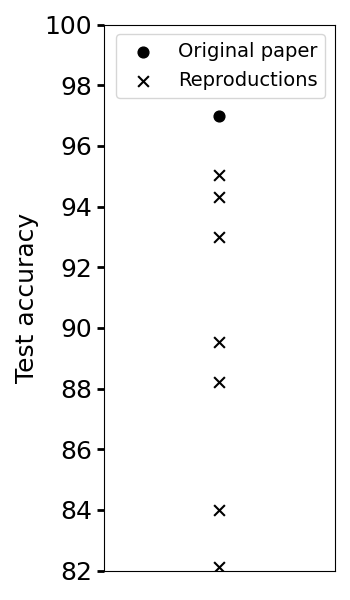
\includegraphics[width=0.40\textwidth]{images/EWCs.png}
    \caption{Summary of the results we identified in the litterature about EWC on 10 tasks p-MNIST benchmarks [REFLA].}
    \label{fig:EWCs}
\end{figure}

\vspace{2mm}
\noindent
Remarkably, all the papers reporting results above or equal to $90\%$ accuracy on the 10 tasks p-MNIST benchmark are either performing a cheated HPO or not explaining their HPO procedure. In particular, the original paper mention that the size of the hidden layers is an optimizable hyperparameter. However, the size of the model does not change when training on the benchmark. This suggests that the HPO performed by the authors of the original paper covers the entire benchmark, that is, the HPO is very likely cheated and include $O(n)$ hyperparameters. See \ref{tab:HPOs} top-center.


\subsection{Validation}


Actually, what we refere to as "cheated HPO" where a single HPO is performed through all the tasks at the same time, could be just fine if one was performing the HPO on a benchmark, and then showing the performances of the approach on another benchmark with the same hyperparameters. Such an approach wouln't even break the hypothesis according to which we do not know the number of tasks in advance. On would just have to perform the HPO on a benchmark with a huge number of tasks, and then show the performances of the approach on another benchmark, with less tasks, using only the hyperparameters computed for the first tasks of the HPO benchmark.

\vspace{2mm}
\noindent
Therefor, we introduce a validation paradigm on benchmarks to measure overfitting on benchmarks. We perform HPO on a benchmark and then measure the drop of performance on another benchmark. However, one could argue that performing HPO on a benchmark like p-MNIST and validating the approach using optimized hyperparameters on a benchmark derivated from CIFAR, for instance, would not be fair. And in order to avoid defining a brittle and handcrafted metric complexity or similarity between benchmarks, we will stick to p-MNIST benchmarks. Indeed, this validation paradigm we are introducing is one of the reasons why we chose to use p-MNIST benchmarks in the first place. Just as we did in \ref{fig:p-MNIST}, we generate $10$ additional p-MNIST benchmarks, each with $10$ tasks. As a consequence, we have benchmarks that sahre the same complexity and similarity from a statistical point of view. We do not perform any HPO on these validation benchmarks. Instead, we reuse the hyperparameter found on the previous benchmark, and simply retrain GroHess with them on the validation benchmarks. See \ref{fig:val_accs_matrix} and \ref{fig:accuracy_through_benchmarks} for the results of this validation paradigm.

\begin{figure}
    \centering
    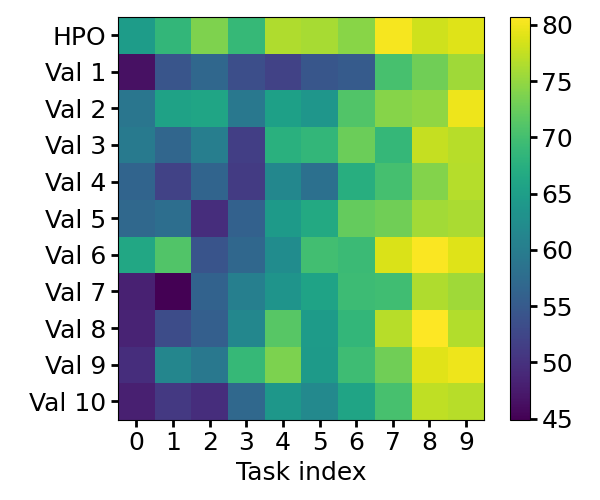
\includegraphics[width=0.4\textwidth]{images/val_accs_matrix.png}
    \caption{Test accuracy on each task once training with GroHess is complete on all the tasks.}
    \label{fig:val_accs_matrix}
\end{figure}

\vspace{2mm}
\noindent
For the HPO benchmark and each of the 10 validation benchmarks, \ref{fig:val_accs_matrix} shows the test accuracy on each task once training with GroHess is complete on all the tasks. These results are run and averaged over seeds 88 to 92. At first glance, it seems that the performance on old tasks are better for the HPO benchmark, suggesting that it is harder for the model to mitigate catastrophic forgetting if the hyperparameters have not been specifically tuned on the benchmark. To confirm this, for each task, we compute the average test accuracy through the validation benchmarks (column wise average) and report the results in \ref{fig:accuracy_through_benchmarks}. In addition, this figure shows the standard deviation for performances on the validation benchmarks, along with the performances obtained on the HPO benchmark (left plot). The right plot shows the same results, averaged out over all tasks. We observe that the average test accuracy over all the tasks of the HPO benchmark are greater by an amount up to $9\%$ than the averge one on the validation benchmarks. This figure confirms that, despite the fact all the benchmarks have the same complexity, performing an HPO on a benchmark is necessary to get the best performances. In other words, GroHess lack of versatility and is overfitting on the benchmark through the HPO process.

\begin{figure}
    \centering
    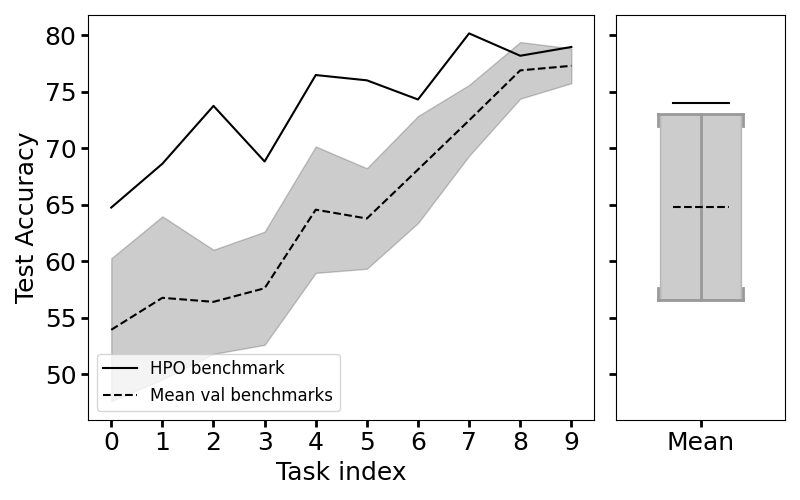
\includegraphics[width=0.45\textwidth]{images/accuracy_through_benchmarks.png}
    \caption{Results from \ref{fig:val_accs_matrix} averaged over the valdiation benchmarks (left plot) and additionally averaged over all tasks (right plot).}
    \label{fig:accuracy_through_benchmarks}
\end{figure}

\vspace{1mm}
\noindent
These results show that the choice of hyperparameters is at the very core of the performances of our method. It means that catastrophic forgetting is mitigated through very specific arbitrations of how the model should learn from new tasks as they come, that is, it seems that our method relies on tradeoffs.



\section{Critical comparison to litterature}



In the following section, we will develop remarks about the methods fitting with our hypothesis. This will a opportunity to compare GroHess to other modular memoryless and unconstrained methods. 


\subsection{Tradeoffs in continual learning}


In the last section, we aknwoledged that the hyperparameter optimization performed in the context of continual learning yield numerous hyperparameters. This can be an implicit way to perform trade-offs between how much the model should learn from the new task versus how much it should remember from the previous tasks. This lead has been confirmed through validation experiments, where we have seen that the very subtle differences between p-MNIST benchmarks are enough to impact the perfomances by an amount of $9\%$. As a consequence, we hypothesize that the HPO procedure is performing tradeoffs between the tasks.

\vspace{2mm}
\noindent
An interesting way to investigate this hypothesis is to have a look at the specific hyperparameters retained by the HPO. Figure \ref{fig:best_params} shows the best values of the hyperparameters found by the HPOs ran on each task of the HPO benchmark. We observe that the learning rate is decreasing by over an order of magnitude as the model moves forward through the tasks. Similarly, we note that the best number of epochs used to train on a task was the highest allowed for the first tasks, and then quickly decreased for the latter tasks. As a consequence, the model model is learning less and less of each tasks. Now we interpret this behavior as a attempt to keep track on previously acquired knowledge while learning on the new task. That is, our approach is mitigating catastrophic through tradeoffs between the specificities of the tasks. As the defenrences between the specifities of the tasks rely on the permutations used to generate the tasks, our interpretation provides an explanation why the model is overfitting on the HPO benchmark. Indeed, the tradeoffs necessary to perform well on a given validation benchmark would require other hyperparameters than the ones found on the HPO benchmark.

\begin{figure}
    \centering
    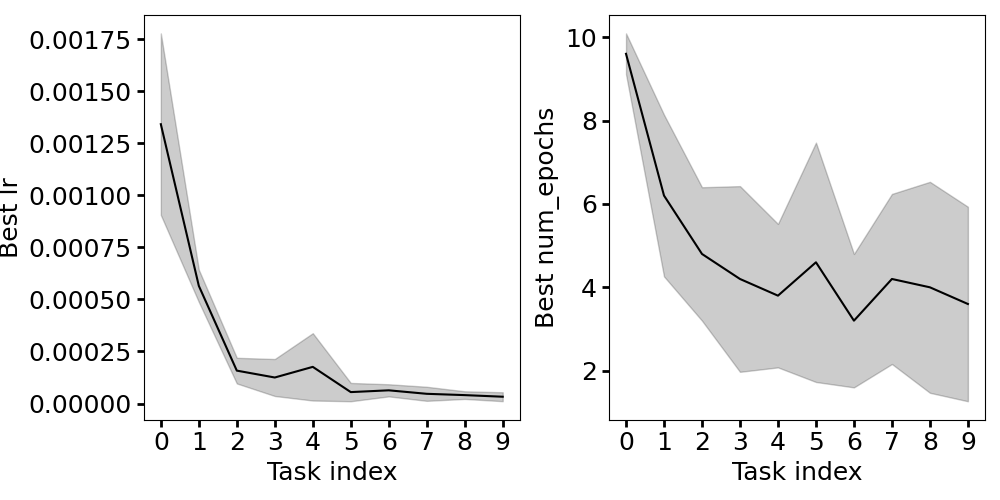
\includegraphics[width=0.5\textwidth]{images/best_params.png}
    \caption{Best values of the hyperparameters (learning rate on the left and number of epochs on the right) found by the HPOs ran on each task of the HPO benchmark.}
    \label{fig:best_params}
\end{figure}

\vspace{2mm}
\noindent
Furthermore, in addition to making tradeoffs between learning and memory for each pair of tasks, methods like GroHess and those based on regularization, such as EWC, SI, LwF or AFEC [REFLA], incorporate trade-offs within the optimization process. Indeed, the regularization term used in these methods is intended to perform tradeoffs between the importance of the new task and the importance of the old tasks. They are controlled by a scalar, which is a hyperparameter is optimized through the HPO procedure. Similarly, through the computation of the Hessian and Gradient masks of importance, GroHess is trading how much to update the weights that are the most crucial for the past tasks versus how much to update these weights for the benefit of the new task. 

\vspace{2mm}
\noindent
Even though all these methods are performing tradeoffs, all the tradeoffs are not the same. From a method to another, the hyperparameters are not the same, which means that the tradeoffs that can be performed through HPO are not the same. This explain the disparities between the results of regularization methods gathered in \ref{fig:results_grouped}. Additionally, the tradeoffs perfomed by regularization methods are continuous, in the sense that they affect all the weights of the model more or less intensively. On the other hand, GroHess performs discrete tradeoffs, only impacting a few weights, leaving the other ones completely unchanged. Finally, to explain results obtained with GroHess that happen to be even poorer than the ones yielded by our baselines, we note that our growing procedure is not optimal. Indeed, it is not embedded in an optimization procedure, as it is the case for the baselines and regularization methods who are optimized through backpropagation only. Thus, it is likely that our growing procedure is simply disturbing the learning process done through backpropagation.


\subsection{Geometrical argument}


In this subsection, we will discuss the geometrical motivation behind several regularization methods such as EWC [REFLA]. Very often, the method is motivated by the representation of a 2-dimensional parameter space, where two ellipses represent regions of low loss when provided data from task A or task B. See \ref{fig:ellipses_EWC}. Once training on task A is done, one assumes that the model is in a state close to the argument of minimum of the loss for data associated to task A, $\theta_A*$. Then, the intuition is that the regularization term introduced in the method will prevent the parameters from converging directly toward the argument of the minimum of the loss for task 2, $\theta_B*$, when learning on task B. Instead, the parameters should converge to an overlapping region where both loss on task A and loss on task B are small. However, this representation is misleading, does not reflect the complexity of the problem and, as a consequence, does not hold in practice. 

\begin{figure}
    \centering
    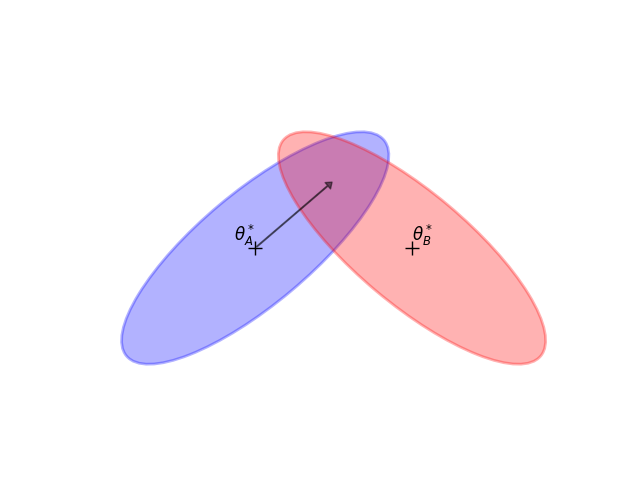
\includegraphics[width=0.45\textwidth]{images/ellipse_overlap.png}
    \caption{Representation of the parameters space as depicted in some regularization papers [REFLA]}
    \label{fig:ellipses_EWC}
\end{figure}

\vspace{2mm}
\noindent
A first objection is that with a regularization method, the direction of parameters modifications does not aim for a minimum of the model trained on the combined data from tasks A and B, but rather towards the local minimum of the model on task B's data that is closest to the local minimum reached by the model trained solely on task A's data.

\vspace{2mm}
\noindent
Second, the Fisher Information Matrix introduced in EWC is leveraged to approximate a metric that indicates what is considered to be the best path to move toward low loss on task $B$, compromising with increase of loss on task A. However, loss on task A is not directly leveraged, as when training on task B, samples from task A are not accessible anymore. As a consequence, authors says that in order to stay close to the region of low loss on task A, it is reasonable to try to update the parameters in a direction of high curvature of the ellipse associated to task A. Indeed, the part of the ellipse that has the highest curvature is also the one that is the furthest from $\theta_A*$, which makes it a direction in which updates of the parameters can be carried without increasing the loss on task A too much. However, contrary to the representaion in \ref{fig:ellipses_EWC}, this is not a guarantee that the model will converge to the center of the overlapping region. Indeed, the overlapping region might not be aligned with the axis passing through $\theta_A*$ and the point of ellipse associated with task A with the highest curvature. See \ref{fig:realistic_ellipses}. In these representation, the red arrow represent the update direction according to $\mathcal{L}_{B}$ and the blue arrow represent the update direction enforced by $\mathcal{L}_{reg}$. The actual update direction is then decided by the value of $\lambda$ and falls inside the cone generated by the two arrows, without covering the whole cone as the linear combination is done through a single scalar. Thus, what matters in the situations depicted in \ref{fig:ellipses_EWC} is the angle between the two arrows along with the orientation of the blue arrow relatively to the red ellipse. The orientation of the red ellipse relatively to the blue arrow accounts for the succes of the update : is the update going to land in a region where both loss on task A and on task B is low ? On the other hand, the angle between the red and the blue arrows accounts for how much $\mathcal{L}_{B}$ and $\mathcal{L}_{reg}$ are acting jointly. In the case depicted in \ref{fig:two_ellipses_45}, no matter what the value of $\lambda$ is, the update will be perfomed toward the overlapping region. This means that the configuration depicted in EWC papers is a really convenient scenario. On the other hand, looking at the configuration in \ref{fig:two_ellipses_90}, we see that the update will be perfomed toward the overlapping region only if the value of $\lambda$ is low enough, because $\mathcal{L}_{reg}$ is pulling the parameters away from the overlapping region. Ultimately, \ref{fig:two_ellipses_180} depicts an extreme scenario, where $\mathcal{L}_{reg}$ is actively acting against $\mathcal{L}_B$. In this configuration, any none zero value of $\lambda$ would make the update worse both with respect to task A and B.

\begin{figure*}
    \centering
    \begin{subfigure}[b]{0.3\textwidth}
        \centering
        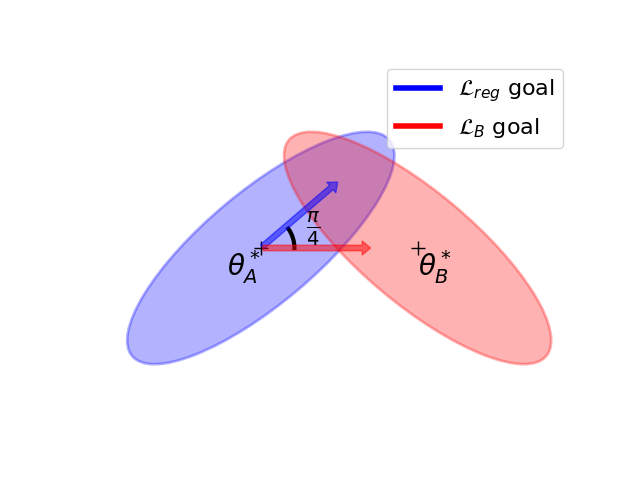
\includegraphics[width=0.99\textwidth]{images/ellipse_overlap_45.png}
        \caption{Configuration depicted in EWC papers}
        \label{fig:two_ellipses_45}
    \end{subfigure}
    \hspace{-0mm}
    \begin{subfigure}[b]{0.3\textwidth}
        \centering
        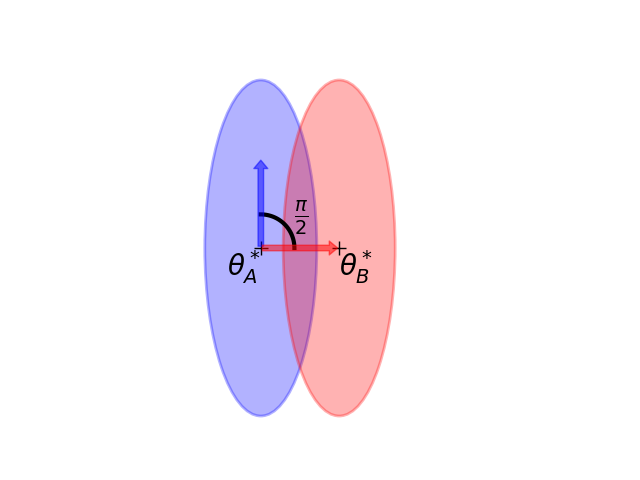
\includegraphics[width=0.99\textwidth]{images/ellipse_overlap_90.png}
        \caption{A configuration less favorable where both the angle and the orientation of the red ellipse are not convenient}
        \label{fig:two_ellipses_90}
    \end{subfigure}
    \hspace{-0mm}
    \begin{subfigure}[b]{0.3\textwidth}
        \centering
        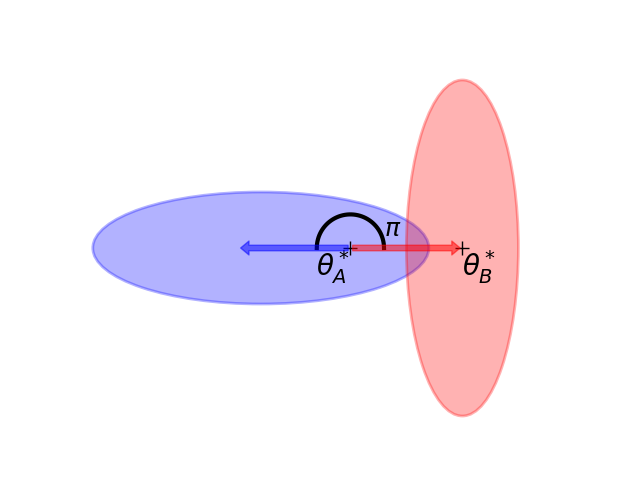
\includegraphics[width=0.99\textwidth]{images/ellipse_overlap_180.png}
        \caption{Extreme configuration where $\mathcal{L}_{reg}$ is actively acting against $\mathcal{L}_B$}
        \label{fig:two_ellipses_180}
    \end{subfigure}
    \caption{Several possible configurations in the parameters space}
\end{figure*}


\vspace{2mm}
\noindent
Furthermore, these illustrations represent a 2-dimensional parameters space, however, in the experiments conducted in the litterature, the parameter space is $\mathbb{R}^n$ with $n \sim 10^5$ or even orders of magnitudes bigger. Additionally, as we already mentionned earlier, the number of tasks in a continual learning benchmark is generally above or equal to $10$, and the research community ultimately expects to be able to tackle as many as hundreds of tasks. As a consequence of these two remarks,the area (or volume) of the overlapping region tends doubly towards 0. On one hand, this representation accounts for two tasks, but in real life scenarios, there are many more. And as the number of tasks increases, the area of the overlapping region decreases, has 0 zero as a lower bound, so converges. But it has no reason to converge toward a non-zero value as the relative position of the low loss ellipses is a priori independant between the tasks, or at least, nobody has provided a better lower bound than 0, to the best of our knowledge. On the other hand, the previous remark implies that there exist a number of tasks for which the overlapping region of interest is small enough to fit within an Euclidean sphere whose radius is strictly smaller than 1, which volume, therefore, converges toward 0 as the dimension of the parameters space increases. 

\vspace{2mm}
\noindent
So, an increase in the number of tasks makes it less likely to find a region where the loss is low for all the tasks, while an increase in the number of parameters of the model somewhat pulls the low loss regions appart from each other. These two remarks do not constitute a strict argument against the regularization methods but rather bring to light the fact the motivation behind them is somewhat flawed. Additionally, the explain why litterature report very poor performances of EWC on longer and harder benchmarks than p-MNIST [REFLA]. Overall, our remarks mostly point out the absence of guarantees. The absence of guaranty is not dramatic though, as deep learning tends to be able to perform well in practice without strong theoretical results. But what is more problematic is that authors of modular, memoryless and unconstrained methods generally do not even have control over the object of our remarks, such as the relative position of the ellipses.

\vspace{2mm}
\noindent
Finally, the worse inherent limitations of modular, memoryless and unconstrained methods is beautifully captured on the \ref{fig:ellipses_EWC} :
\begin{quote}
    \itshape
    \centering
    Improving on task B means deteriorating on task A, and reciprocally.
\end{quote}
\vspace{2mm}
\noindent
It does not mean that the more tasks there are to solve, the harder it gets to solve them all, which is true. Our statement is stronger, it means that tasks are inhrently put in a competition setting with each other. This implies that performing continual learning with modular, memoryless and unconstrained methods inherently boils down to perform tradeoffs, which confirms our prior analysis of tradeoffs through HPOs. Ultimately, it imlpies that modular, memoryless and unconstrained methods are inherently limited when it comes to perform continual learning on numerous tasks. By contrast, we do not find this inherent limitation with in Mixture of Experts models [REFLA], where modules dedicated to each tasks are in parallel, and improving one particular module does not hurt another module as long as the gating system remains the same. And this gating system can be implemented using replay or rehearsal methods, or leveraging feature extractor such as CNN masks. But here we break one of our two assumptions: either we leverage some form of memory or we employ architectural constraints.


\subsection{Combinatorial argument}


\vspace{1mm}
\noindent
Let's assume we are given $I$ tasks indexed in increasing order by the set $\intset{1}{I}$. We define a neural network as the set of its parameters
\begin{align}
    \phi = \left\{\left\{ w_{l,m,n} \in \mathbb{R} | m,n \in \llbracket 1, N_{l-1} \rrbracket \times \llbracket 1, N_{l} \rrbracket \right\} | l \in \llbracket 1, L+1 \rrbracket \right\}
\end{align}
where $L$ is the number of hidden layers and $N_l$ is the number of neurons on layer $l$.

\vspace{1mm}
\noindent
Let's define $\mathbb{W}_{l,n}^i$ to be the set of protected weights for task $i$ with respect to neuron $n$ of layer $l$, for any $i \in \intset{1}{I}$, $l \in \intset{1}{L+1}$ and $n \in \intset{1}{N_l}$:
\begin{align}
    \mathbb{W}_{l,n}^i = \left\{ w_{l,m,n}, m \in \intset{1}{N_{l-1}} | w_{l,m,n} \text{ protected} \right\}
\end{align}

\vspace{1mm}
\noindent
which allows to define the pollution of task $i$ by protected weights for task $j$ on neuron $n$ of layer $l$ as
\begin{align}
    p_{l,n}^{i\rightarrow j} = \mathbb{E}_{x \sim D_i}\left[\frac{\sum_{w \in \mathbb{W}_{l,n}^j}{w(x)}}{\sum_{w \in \mathbb{W}_{l,n}^i}{w(x)}}\right]
\end{align}

\vspace{1mm}
\noindent
Finally, we can define the pollution of task $i$ by protected weights for task $j$ on the whole network as
\begin{align}
    P^{i\rightarrow j} = \frac{1}{L+1}\sum_{l=1}^{L+1}{\frac{1}{N_l}\sum_{n=1}^{N_l}{p_{l,n}^{i\rightarrow j}}}
\end{align}

\begin{table}
\begin{tabular}{|c|c|c|}
    \hline
    \diagbox{{\footnotesize Tested}}{{\footnotesize Trained}} & Taks 1 & Task 2 \\ \hline
    Task 1 & 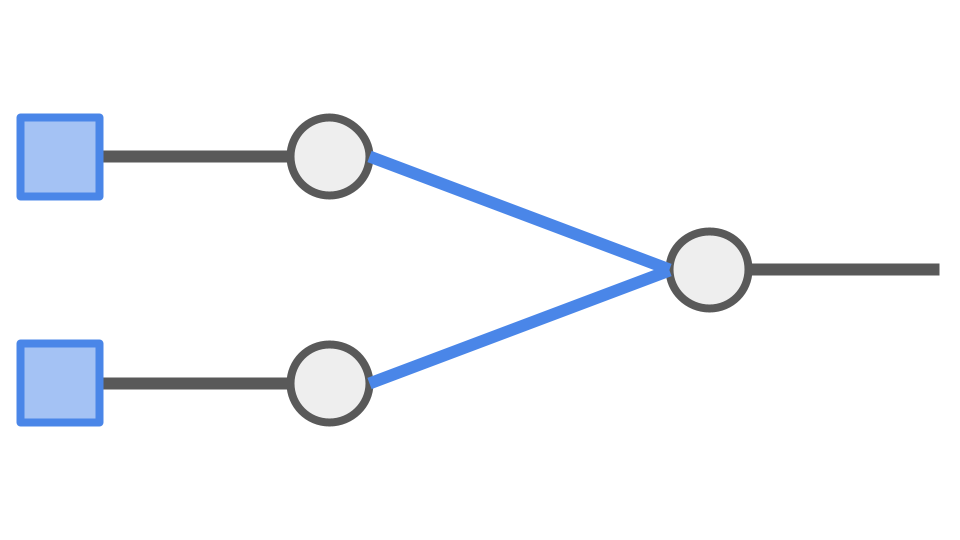
\includegraphics[width=2.5cm]{images/pollution_11.png} & 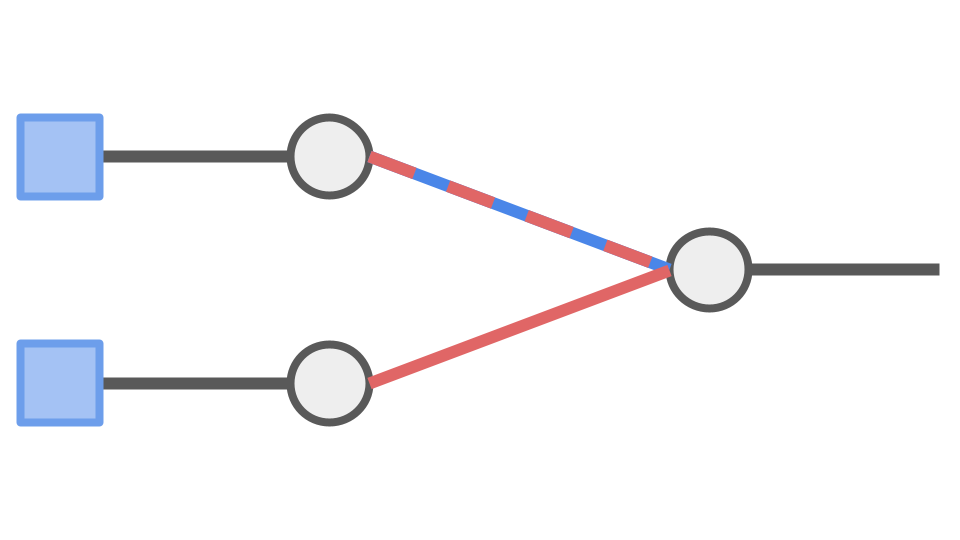
\includegraphics[width=2.5cm]{images/pollution_12.png} \\ \hline
    Task 2 & \notableentry & 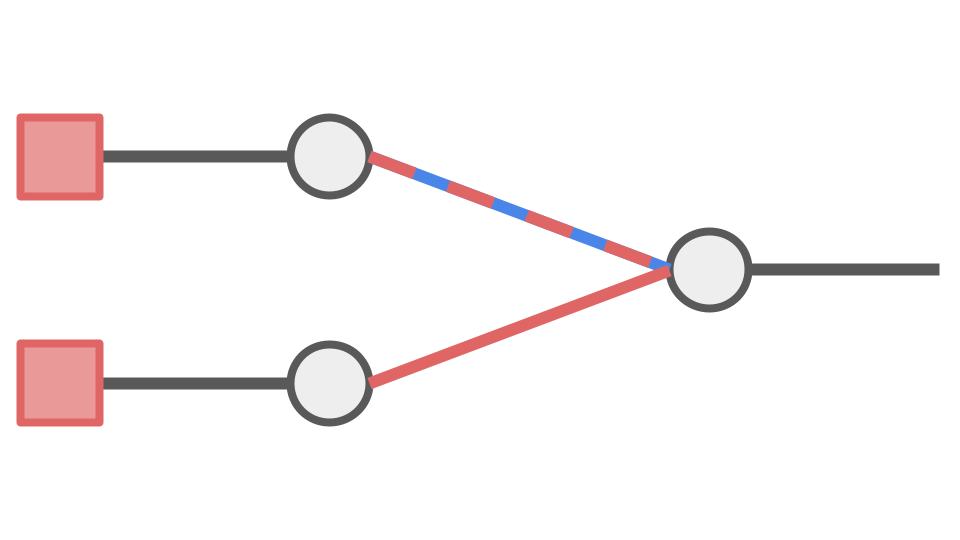
\includegraphics[width=2.5cm]{images/pollution_21.png} \\ \hline
\end{tabular}
\caption{After training on task 1, there is no pollution (top left). After training on task $2$, there is $P^{1\rightarrow 2}$, pollution from task-2-specific weights when forwarding task 1 samples (top right) and $P^{2\rightarrow 1}$, pollution from task-1-specific weights when forwarding task $2$ samples (bottom right).}
\label{table:pollution}
\end{table}


\vspace{1mm}
\noindent
The notion of pollution $P^{i\rightarrow j}$ encapsulates how much neurons specialized for a task $j$ interfere whith neurons specialized for a task $i$ when provided a sample from task $i$, after training on the first $\max(i,j)$ tasks at least. See \ref{table:pollution} for a simple illustration. Once the model is trained on task 1, we can test it on data from task 1 (top left cell) but we can't expect it to perform well on data from the next tasks (bottom left cell), so no pollution is occuring. Once the model is trained on task 2, we expect it to perform well on task 1 and 2, so the pollutions that can occur are $P^{2\rightarrow 1}$ (top right cell) and $P^{1\rightarrow 2}$ (bottom right cell). $P^{2\rightarrow 1}$ is generally handled by regularization approaches that keep certain weights of the model close to the weights of the model after training on task 1. The training process on task 2 take into consideration these dedicated weights, and the model learns to forward samples from task 2 through all the weights. However, $P^{1\rightarrow 2}$ is not handled by these approaches, as the model can't learn how to forward samples from task 1 through the undedicated weights retrained on task 2.

\vspace{1mm}
\noindent
More boradly, the challenge is to deal with $P^{i\rightarrow j}$ for $j \neq i$, which requires to learn data from task $i$ without being polluted by data from task $j$. Regularization approaches such as EWC claim to solve pollution of task $j$ over task $i$ $(P^{i\rightarrow j}=0)$ for $j<i$. While they can't really overcome it, they can at least mitigate it by penalizing the distance between the weights of the model after training on task $i$ and the weights of the model after training on task $j$. However, they do not tackle the minimization of $P^{i\rightarrow j}$ for $j>i$. But they have a good reason no to tackle it : this is a fundamental limitation of this familly approaches, as it is inherently not possible to deal with it. Indeed, without contraints or some form of memory of the previous tasks, when provided a sample from task $i$, the model has no discrimination power of weights updated for task $j$ from the ones the approach identified as specific for task $i$ when training on task $j$, for $j>i$. So it can't know how to react to a sample from task $i$ after training on task $j>i$.

\vspace{1mm}
\noindent
Conversely, allowing some form of memorization of previous data distribution may enable to discriminate between samples features. This is has been attempted through replay memory approaches \cite{replay1}, \cite{replay2} and rehearsal methods \cite{rehearsal}. Alternatively, it can also be achieved through gating mechanisms such as mixture of expert models \cite{moe}, \cite{dmoe}. These approaches are not memoryless. However, in memoryless approaches we have no direct control over the way the neurons specialized to task $j$ will react when fed with samples from task $i<j$. So the very last hopes without memory is that the weights are such that they implicitly encode information about the task's specificities. This can be performed with constrained models, such as CNN, through which one could enforce convolution kernels associated to one task to be orthogonal to the convolution kernels associated to another task. And with additional contraints, this would prevent the model from using the same features for two different tasks while selecting for the most relevant features for each task. But, we considere unconstrained approaches, so the model has no reason to encourage such behavior.





\section{Additional remarks and opening}
% GradMax
% Usecases
% DANN


\section{Conclusion}



In the end, this efforts put in writting this paper beautifully illustrate Brandolini's law : 
\begin{quote}
    The amount of energy needed to refute bullshit is an order of magnitude bigger than that needed to produce it
\end{quote}
We corrected the work subsequent to two small mistakes, namely, that could have been avoided by a more careful preliminary analysis of the problem. The fact that a method relies on an attempt to balance how much we hurt the learning process on each task naturally introduces trade-offs. These trade-offs are performed through hyperparameters in the loss that set the relative importance of the task, which can easily be mismanipulated or lead to overfitting on the benchmarks at hand.


\vspace{1mm}
\noindent
Finally, it appears that manipulation of hyperparameters in the context of continual learning is subtle, and we encourage more care in their management.



\nocite{*}
\printbibliography



\end{document}







\subsection{Continual learning usecases}

We already argued that continual learning is not a well-defined problem. In this section, we will question the very fundamental assumption of continual learning. and it is not clear what are the usecases of continual learning.

Here is a list each and every usecase of continual learning :
\begin{itemize}
    \item Adapt to new data quickly https://neptune.ai/blog/continual-learning-methods-and-application
        \begin{itemize}
            \item Bank fraud (want to adapt quickly to new method)
        \end{itemize}
    \item A model needs to be personalized https://neptune.ai/blog/continual-learning-methods-and-application
        \begin{itemize}
            \item Let’s say you maintain a document classification pipeline, and each of your many users has slightly different data to be processed—for example, documents with different vocabulary and writing styles. With continual learning, you can use each document to automatically retrain models, gradually adjusting it to the data the user uploads to the system.
        \end{itemize}
\end{itemize}

Remarks :
\begin{itemize}
    \item For bank fraud, we don't have enough knowledge to formulate objections.
    \item Model personalization sounds like finetuining, not continual learning... does it make sense to try to train a single model that we want to use on every client ? Isn't it better to do it in the LoRA fashion, and fine-tune a module that we store with the  client's data ?
\end{itemize}




\vspace{1mm}
\noindent
Overcomplexification : In AFEC: Active Forgetting of Negative Transfer in Continual Learning, they introduce a new term in the loss, with a new hyperparameter "while the forgetting factor regulates a penalty to selectively merge the main network parameters with the expanded parameters, so as to learn a better overall representation of both the old tasks and the new task.", so they are trying to mitigate the mitigation made by a regularization method such as EWC. Additionnaly, they hope "to learn a better overall representation of both the old tasks and the new task", which has no reason to happen without enforcing such behavior through constraints, which they don't do.





%========================================================
% Old cheated HPO
\begin{table}[h!]
    \centering
    \begin{tabular}{cc}
        \begin{tabular}{c|ccc|}
            \hline
            Data from & $T_1$ & $\cdots$ & $T_m$ \\ \hline
            \multirow{3}{*}{HP at hand} & \multicolumn{3}{c|}{$h_1$} \\
            & \multicolumn{3}{c|}{$\vdots$} \\
            & \multicolumn{3}{c|}{$h_m$} \\ \hline
        \end{tabular}
        &
        \hspace{-5mm}
        \begin{tabular}{c}
                                                    \\
                                                    \\
                                                    \\
            \hspace{-1.5mm}\footnotesize{$HPO$}\\
        \end{tabular}
    \end{tabular}
    \caption{Cheated HPO : $O(1)$ parameters}
    \label{tab:cheated_hpo}
\end{table}




%========================================================
% Cheated HPO
\begin{table}[h!]
    \centering
    \begin{tabular}{cc}
        \begin{tabular}{c|ccc|}
            \hline
            Data from & $T_1$ & $\cdots$ & $T_m$ \\ \hline
            HP at hand & \multicolumn{3}{c|}{$\lambda_1$} \\\hline
        \end{tabular}
        &
        \hspace{-5mm}
        \begin{tabular}{c}
                                                    \\
                                                    \\
                                                    \\
            \hspace{-1.5mm}\footnotesize{$HPO$}\\
        \end{tabular}
    \end{tabular}
    \caption{Cheated HPO : $O(1)$ parameters}
    \label{tab:cheated_hpo1}
\end{table}


%========================================================
% Old greedy HPO
\begin{table*}[h!]
    \centering
    \begin{tabular}{cccccc}
        \begin{tabular}{|c|}
            \hline
            $T_1$    \\\hline
            $h_1^1$  \\
            $\vdots$ \\
            $h_m^1$  \\\hline
        \end{tabular}
        &
        \hspace{-6mm}
        \begin{tabular}{c}
                                                \\
            \hspace{2mm} $\longrightarrow$      \\
                                                \\
            \hspace{-3mm}\footnotesize{$HPO_1$} \\
        \end{tabular}
        &
        \hspace{-4mm}
        \begin{tabular}{|c|}
            \hline
            $T_2$    \\\hline
            $h_1^2$  \\
            $\vdots$ \\
            $h_m^2$  \\\hline
        \end{tabular}
        &
        \hspace{-6mm}
        \begin{tabular}{c}
                                                                          \\
            \hspace{2mm} $\longrightarrow$ \ldots $\longrightarrow$       \\
                                                                          \\
            \hspace{-14mm}\footnotesize{$HPO_2$}                          \\
        \end{tabular}
        &
        \hspace{-4mm}
        \begin{tabular}{|c|}
            \hline
            $T_n$    \\\hline
            $h_1^n$  \\
            $\vdots$ \\
            $h_m^n$  \\\hline
        \end{tabular}
        &
        \hspace{-6mm}
        \begin{tabular}{c}
                                                 \\
                                                 \\
                                                 \\
            \hspace{-1.5mm}\footnotesize{$HPO_n$}\\
        \end{tabular}
    \end{tabular}
    \caption{Greedy HPO : $O(n)$ to $O(n^2)$ parameters}
    \label{tab:greedy_hpo}
\end{table*}


%========================================================
% Greedy HPO n
\begin{table*}[h!]
    \centering
    \begin{tabular}{cccccc}
        \begin{tabular}{|c|}
            \hline
            $T_1$    \\\hline
            $\emptyset$  \\\hline
        \end{tabular}
        &
        \hspace{-6mm}
        \begin{tabular}{c}
                                                \\
            \hspace{2mm} $\longrightarrow$      \\
                                                \\
            \hspace{-3mm}\footnotesize{$HPO_1$} \\
        \end{tabular}
        &
        \hspace{-4mm}
        \begin{tabular}{|c|}
            \hline
            $T_2$    \\\hline
            $\lambda_2$  \\\hline
        \end{tabular}
        &
        \hspace{-6mm}
        \begin{tabular}{c}
                                                                          \\
            \hspace{2mm} $\longrightarrow$ \ldots $\longrightarrow$       \\
                                                                          \\
            \hspace{-14mm}\footnotesize{$HPO_2$}                          \\
        \end{tabular}
        &
        \hspace{-4mm}
        \begin{tabular}{|c|}
            \hline
            $T_n$    \\\hline
            $\lambda_n$  \\\hline
        \end{tabular}
        &
        \hspace{-6mm}
        \begin{tabular}{c}
                                                 \\
                                                 \\
                                                 \\
            \hspace{-1.5mm}\footnotesize{$HPO_n$}\\
        \end{tabular}
    \end{tabular}
    \caption{Greedy HPO : $O(n)$ parameters}
    \label{tab:greedy_hpo1}
\end{table*}






%========================================================
% Greedy HPO n^2
\begin{table*}[h!]
    \centering
    \begin{tabular}{cccccccc}
        \begin{tabular}{|c|}
            \hline
            $T_1$    \\\hline
            $\emptyset$  \\\hline
        \end{tabular}
        &
        \hspace{-6mm}
        \begin{tabular}{c}
                                                \\
            \hspace{2mm} $\longrightarrow$      \\
                                                \\
            \hspace{-3mm}\footnotesize{$HPO_1$} \\
        \end{tabular}
        &
        \hspace{-4mm}
        \begin{tabular}{|c|}
            \hline
            $T_2$    \\ \hline
            $\lambda_{2,1}$ \\ \hline
        \end{tabular}
        &
        \hspace{-6mm}
        \begin{tabular}{c}
                                                \\
            \hspace{2mm} $\longrightarrow$      \\
                                                \\
            \hspace{-3mm}\footnotesize{$HPO_2$} \\
        \end{tabular}
        &
        \hspace{-4mm}
        \begin{tabular}{|c|}
            \hline
            $T_3$    \\ \hline
            $\lambda_{3,1}$ \\
            $\lambda_{3,2}$ \\ \hline
        \end{tabular}
        &
        \hspace{-6mm}
        \begin{tabular}{c}
                                                                          \\
            \hspace{2mm} $\longrightarrow$ \ldots $\longrightarrow$       \\
                                                                          \\
            \hspace{-14mm}\footnotesize{$HPO_3$}                          \\
        \end{tabular}
        &
        \hspace{-4mm}
        \begin{tabular}{|c|}
            \hline
            $T_n$    \\\hline
            $\lambda_{n,1}$  \\
            $\vdots$ \\
            $\lambda_{n,n-1}$  \\\hline
        \end{tabular}
        &
        \hspace{-6mm}
        \begin{tabular}{c}
                                                 \\
                                                 \\
                                                 \\
            \hspace{-1.5mm}\footnotesize{$HPO_n$}\\
        \end{tabular}
    \end{tabular}
    \caption{Greedy HPO : $O(n^2)$ parameters}
    \label{tab:greedy_hpo2}
\end{table*}